%The fwahl LaTeX template made for use at TU Eindhoven

\documentclass[11pt, a4paper, onecolumn, oneside, parskip=half]{scrartcl}

%%%%%%%SETUP BEGIN%%%%%%%
%Define constant names, etc.
\newcommand{\authors}{\\Stef Louwers (0590864)\\
Sunil Chokkanathapuram Ramanarayanan (0826874)\\
Qian Qian (0827493)\\
GROUP 3
} %List Authors here
\newcommand{\prof}{Prof. dr. Henk Corporaal, Mark Wijtvliet, MSc} %List Prof here
\newcommand{\doctitle}{Design and Implementation of a Quadcopter with Visual Control} %Document Title
\newcommand{\subcode}{5HC99} %Subject Code
\newcommand{\docsubject}{Embedded Visual Control} %Subject name, also appears in header
\newcommand{\centerhead}{S.T.Louwers, S.Chokkanathapuram Ramanarayanan, Q.Qian} %Center part of header
\newcommand{\centerfoot}{} %Center part of footer
%%%%%%%SETUP END%%%%%%%%
\usepackage{caption}
%\usepackage{subfigure}
\usepackage{subcaption}
\usepackage{graphicx}
\usepackage{amsmath}
\usepackage{listings}
\usepackage{a4wide}
\usepackage{color}
\usepackage{listings}
\usepackage{float}
\usepackage{amsmath}
\usepackage{booktabs}
\usepackage{footmisc}
\usepackage{sectsty}
\usepackage[headsepline,footsepline]{scrpage2}
\usepackage[hidelinks]{hyperref}
\usepackage{titlesec}
\usepackage{placeins}
\usepackage{textcomp}

% Nonindented footnotes
\setlength{\footnotemargin}{2mm}

% Prevent PDF Version warnings
\pdfminorversion=6

% Colors
\definecolor{darkblue}{rgb}{0.0,0.0,1}
\definecolor{midgreen}{rgb}{0.0,0.5,0.0}
\definecolor{lightgray}{gray}{0.95}

% Listings
\lstset
{
	language=Verilog,
	frame=single,
	backgroundcolor=\color{lightgray},
	showstringspaces=false,
	keywordstyle=\bfseries\color{darkblue},
	commentstyle=\color{midgreen},
	basicstyle=\ttfamily\fontsize{8}{8}\selectfont,
	numbers=left,
	captionpos=b,
	breaklines=true,
	aboveskip=\baselineskip,
	tabsize=2
}

% New commands
\newcommand{\HRule}[2]{\noindent\rule[#1]{\linewidth}{#2}}
\newcommand{\vlinespace}[1]{\vspace*{#1\baselineskip}}
\newcommand{\todo}[1]{{\textcolor{red}{\textbf{TODO:} #1}}}

% TOC
\setcounter{tocdepth}{2}


% Header and footer
\ihead{\docsubject{}}
\chead{}
\ohead{\centerhead{}}
\ifoot{\headmark}
\cfoot{\centerfoot{}}
\ofoot{\thepage}
\automark[section]{section}

% Redefine headings
\titleformat{\section}{\sffamily\large\bfseries}{\thesection}{1em}{}
\titleformat{\subsection}{\sffamily\normalsize\bfseries}{\thesubsection}{1em}{}
\titleformat{\subsubsection}{\sffamily\normalsize\bfseries}{\thesubsubsection}{1em}{}
\titleformat{\paragraph}{\sffamily\normalsize\bfseries}{\theparagraph}{1em}{}
\titleformat{\subparagraph}{\sffamily\small\bfseries}{\thesubparagraph}{1em}{}

\begin{document}

\begin{titlepage}

\sffamily
\hfill \centering

\includegraphics[width=7cm]{tuelogo}
\HRule{11pt}{2pt}

\vfill
\Large{\docsubject{} \\\subcode{} \\}
\vlinespace{1}
\huge{\doctitle{}\\}
\vlinespace{8}
\vfill
\large
By \authors{}\\
\vfill
%\vlinespace{5}
\HRule{11pt}{2pt}
\raggedright
\textbf{Date: } \today \\
\textbf{Professor:} \prof{}

\end{titlepage}

\tableofcontents
\newpage
\pagestyle{scrheadings}

\section{Introduction}
In this project, a quadcopter is designed and implemented to autonomously fly and demonstrate on-board image processing capabilities. The project is aimed to control the quadcopter by virtue of two control systems; the local control, and the global control. The local control is intended for the stabilisation of the quadcopter, so that it is able to fly manually through the RC receiver and the global control is intended to make the quadcopter to fly autonomously with the aid of visual control through the camera. These two control loops are implemented on dedicated processors with appropriate capabilities.

% \section{Requirements}
% \section{Hardware}

\section{System Architecture}
\label{sec:arch}
In this section, we will discuss the used hardware and system architecture. First we will take a look at the local control, global control and used sensors, and after that, we will address communication used between these components.

\subsection{Local Control}
\label{sec:arch:local}
The local control is powered by an STM32F3Discovery development board (figure \ref{fig:stm32f3}), powered by the STM32F303VCT6 processor (a 72 MHz Cortex-M4 MCU), 48 KB RAM and 256 KB flash memory. This board also contains a gyroscope, accelerometer and a magnetic sensor, all measuring three axis. This makes it an ideal board for a quadcopter's local control, because it contains enough processing power, and has all the basic sensors available.

\begin{figure}[ht]
\centering
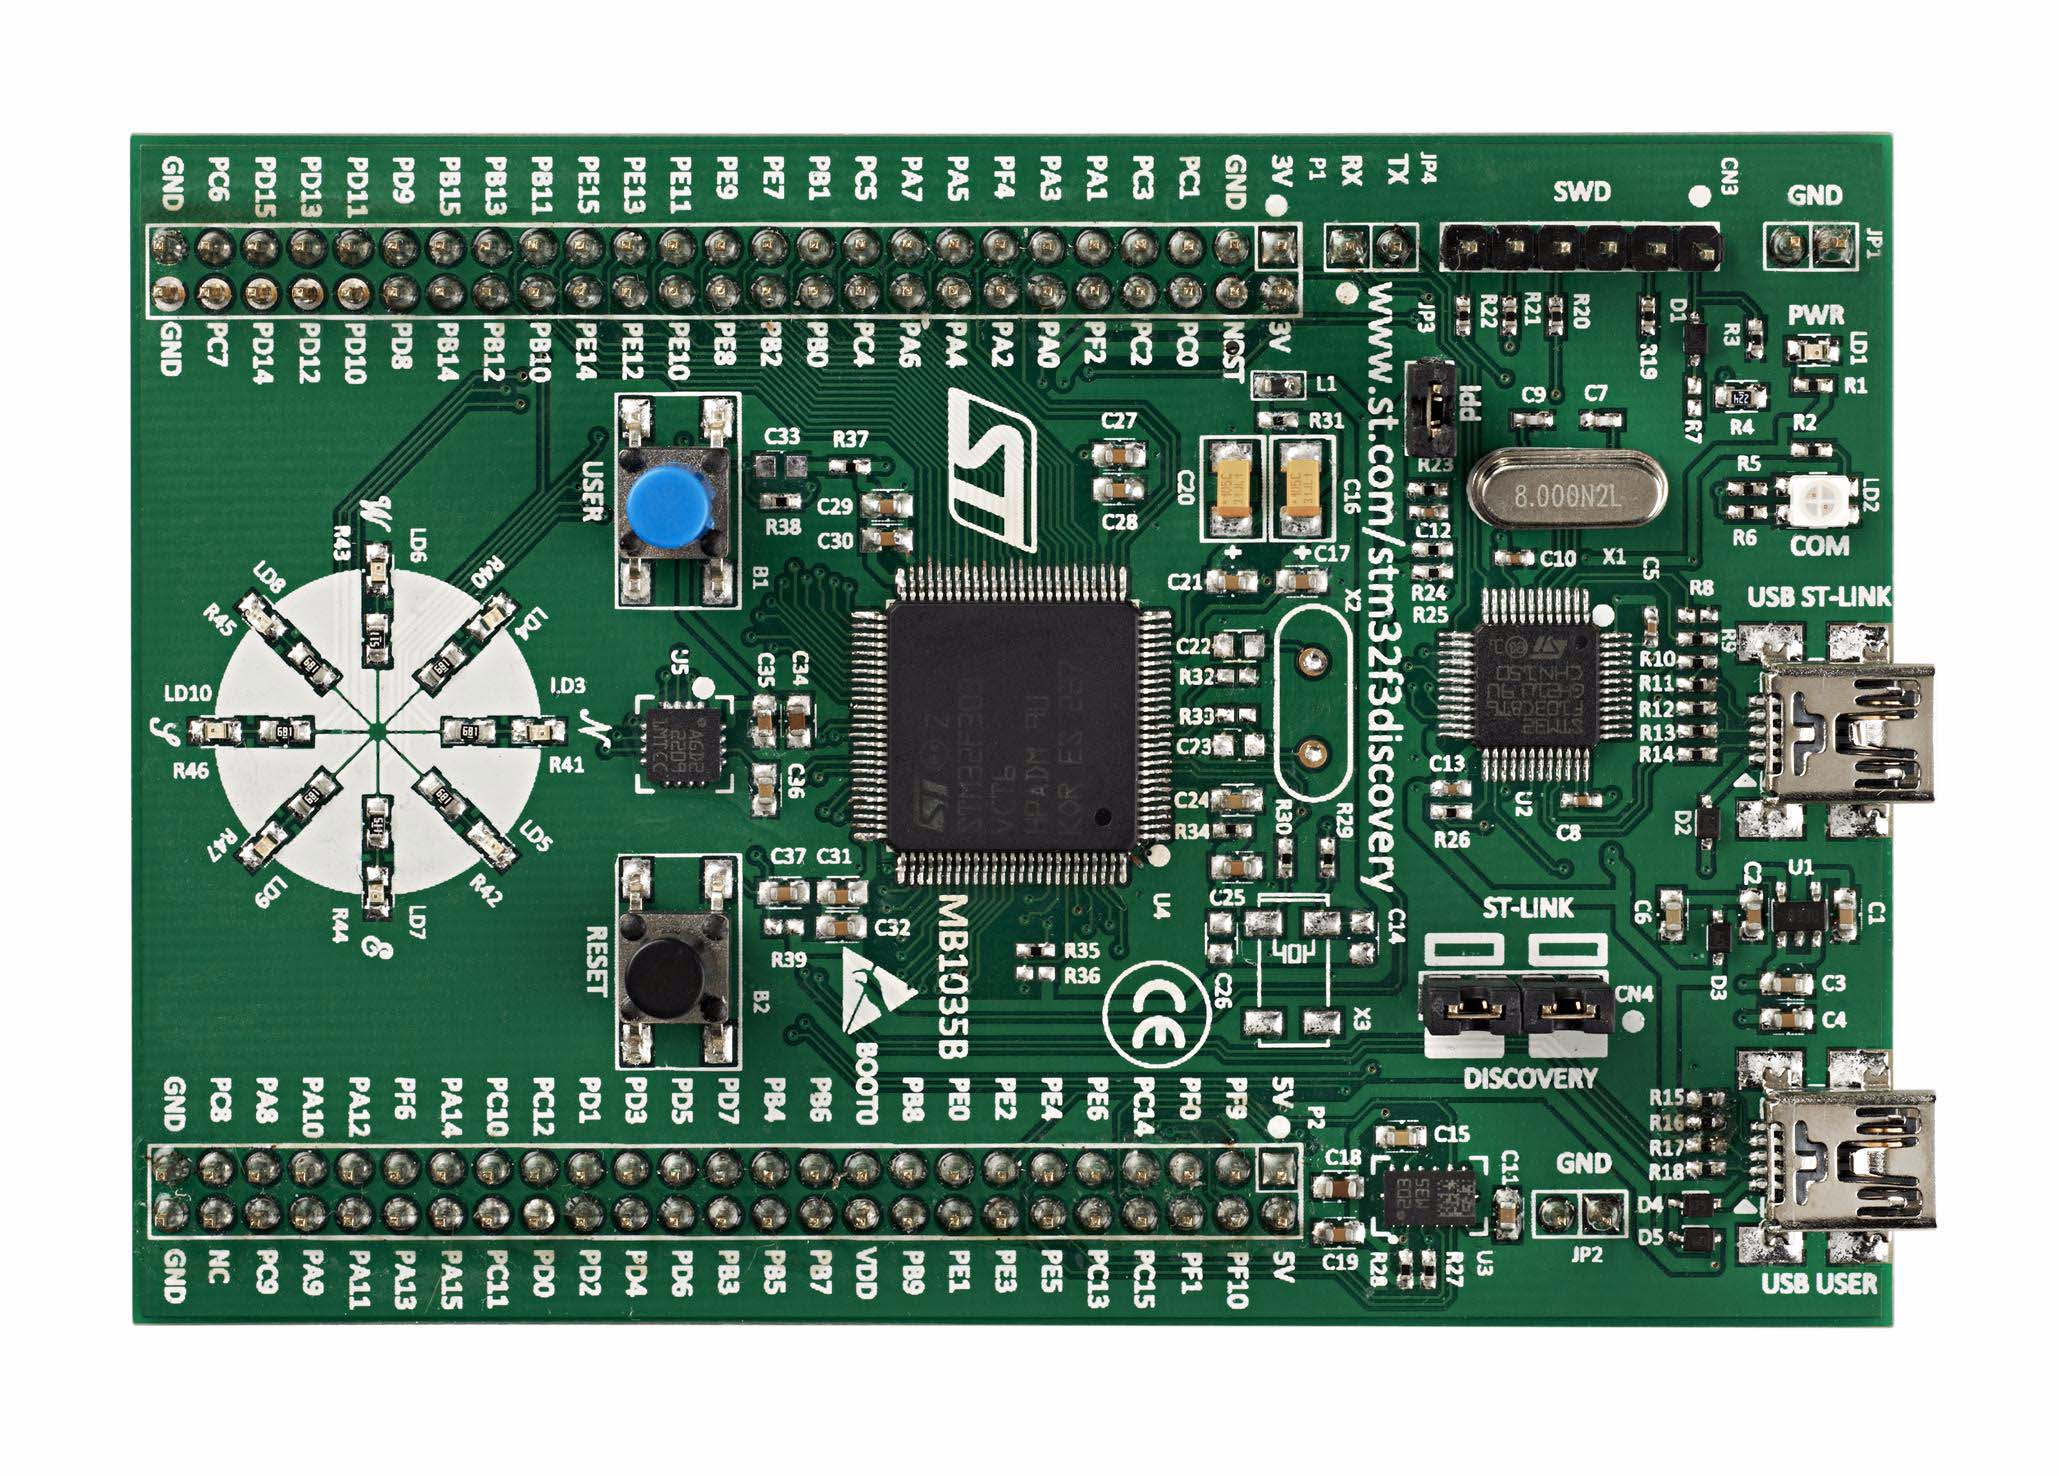
\includegraphics[width=0.6\textwidth]{STM32F3DISCOVERY}
\caption{An STM32F3Discovery.}
\label{fig:stm32f3}
\end{figure}

\subsection{Global Control}
\label{sec:arch:global}
For the global control, we have chosen for the Raspberry PI (figure \ref{fig:raspi}). We chose for this platform because it was cheap, we already had it available, and the camera module was expected soon after the start of the project.

Because we wanted two cameras on the quadcopter (one facing to the front, and one facing down), we decided to add two Raspberry PIs to the quadcopter, as each Raspberry PI only has the possibility to connect one camera. This also gave us more processing power available, as each Raspberry PI only has to process one camera.

\begin{figure}[ht]
\centering
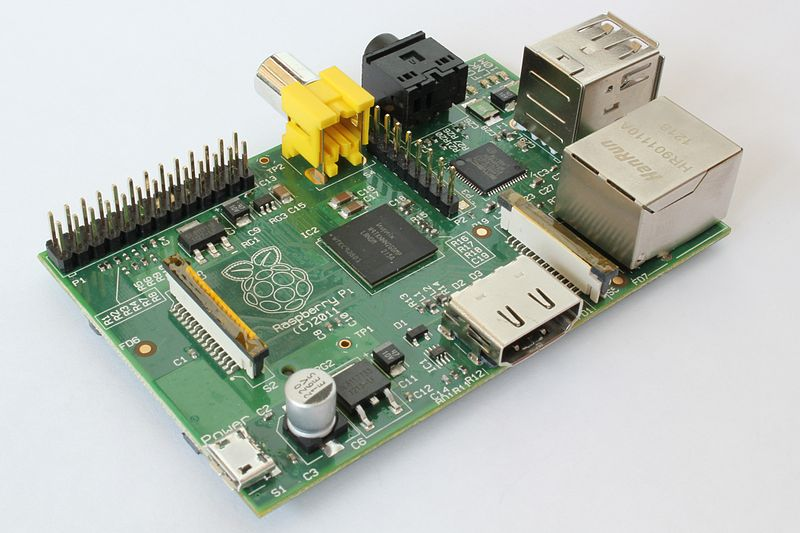
\includegraphics[width=0.6\textwidth]{image01}
\caption{A Raspberry PI.}
\label{fig:raspi}
\end{figure}

\subsection{Sensors}
\label{sec:arch:sensors}
The local control board already contained the basic sensors required to fly a quadcopter: a gyroscope, an accelerometer and a magnetic sensor. To this list, we added a battery monitor, a barometer and two cameras.

\subsubsection{Battery monitor}
\label{sec:arch:sensors:battery}
The battery monitor was a simple voltage divider that connected the battery voltage to one of the ADC pins of the STM32F3Discovery board. The voltage divider was necessary to convert the voltage to the 0 -- 3V domain.

\subsubsection{Ultrasound}
\label{sec:arch:sensors:ultrasound}
Initially the plan was to use the ultrasound sensor (figure \ref{fig:hcsr04}) for tracking the altitude of the quadcopter. The HCSR04 sonar driver was requested from Taulabs development team and merged to our code base. The ultrasound driver implementation could be obtained in Github link\footnote{\url{https://github.com/scenkov/TauLabs}}. As we further realized, the ultrasound sensor suffered propeller sound interference which made the sensor values noisy and inaccurate. This happened because there were high frequency components in the sound waves emitted by the propellers and it fell in the band of 40 KHz which was the operating frequency of the sound waves used for ultrasound sensor, hence this interference resulted in changing our design decision to use alternative altitude tracking sensor such as barometer instead of the ultrasound sensor.

\begin{figure}[ht]
\centering
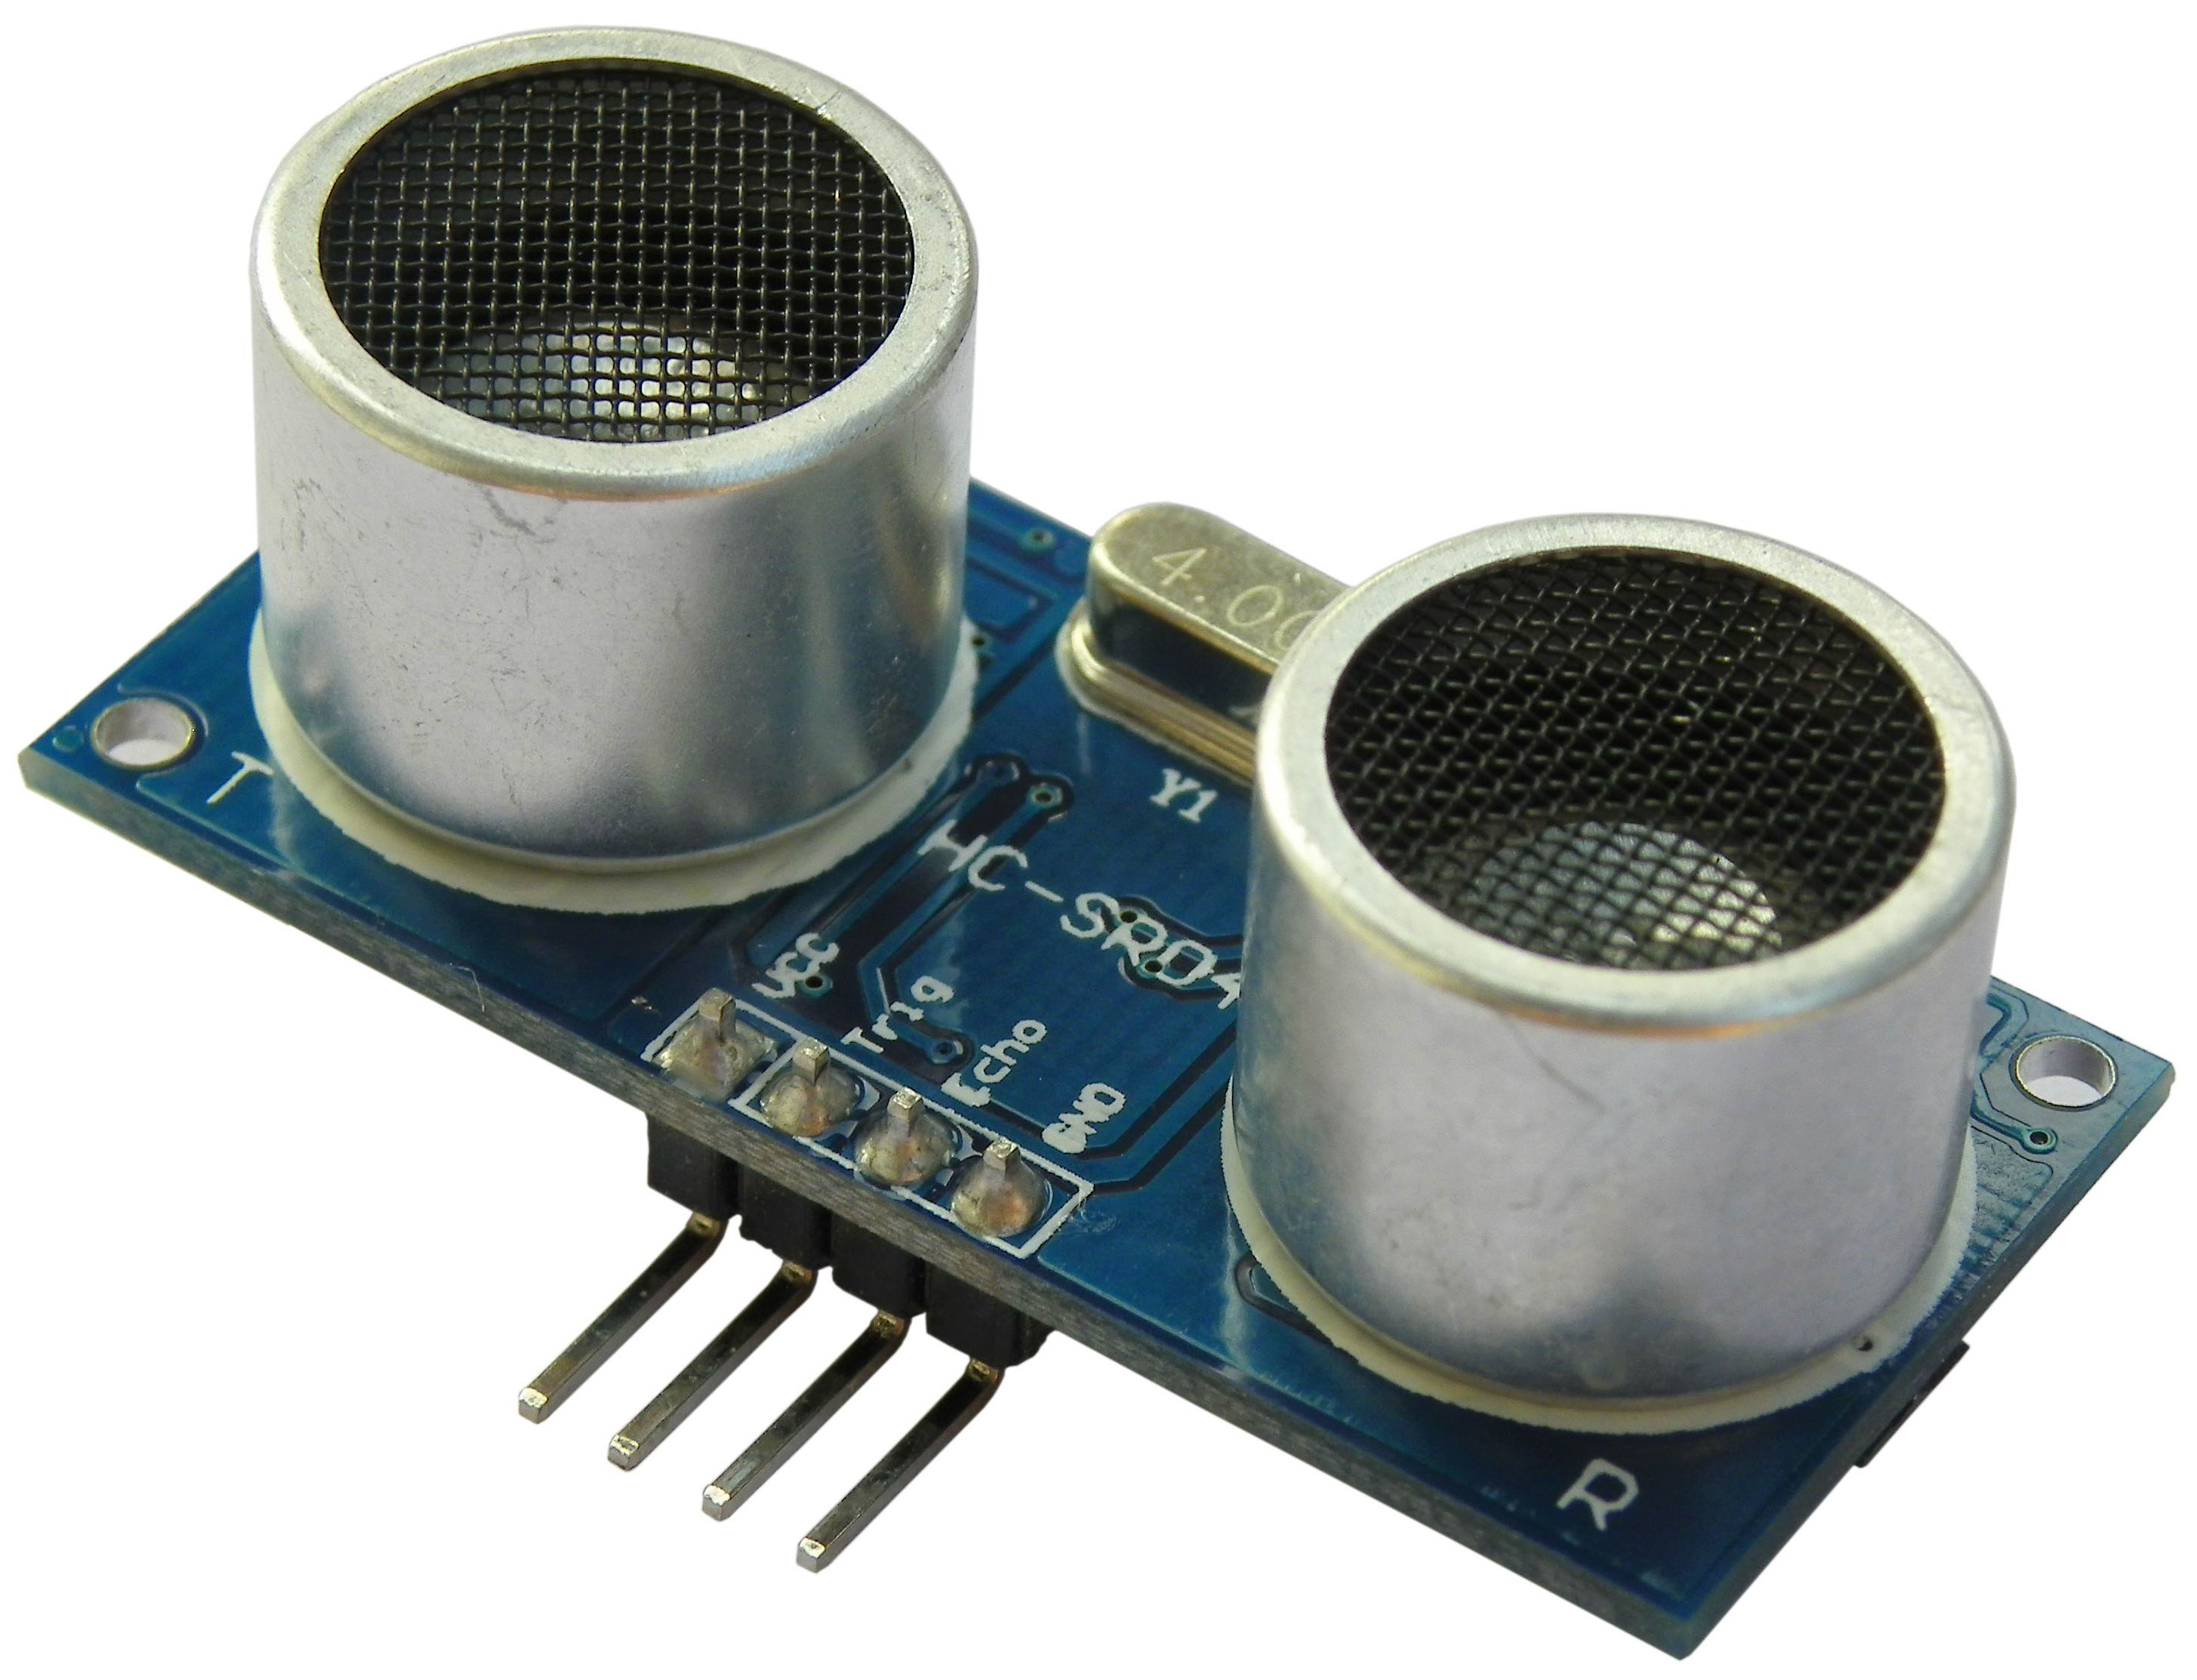
\includegraphics[width=0.3\textwidth]{HC-SR04}
\caption{The HCSR04 sensor.}
\label{fig:hcsr04}
\end{figure}

\subsubsection{Barometer}
\label{sec:arch:sensors:batometer}
In order to facilitate altitude hold, we needed some means of measuring the current altitude of the quadcopter. Because of the problems we and other teams have experienced with the ultrasound sensor, we decided to do something different and try a barometer (figure \ref{fig:BMP085}).

Compared to an ultrasound sensor, a barometer has less accuracy. Also, a barometer provides only a absolute height (to sea level). Thus a command like ``stay at 1 meter from the ground'' is not possible. Instead, we should say ``stay at the current height''. The advantage of the barometer over the ultrasound sensor is that it has no height limits, and that there are no false measurements as reported with the other groups.

\begin{figure}[ht]
\centering
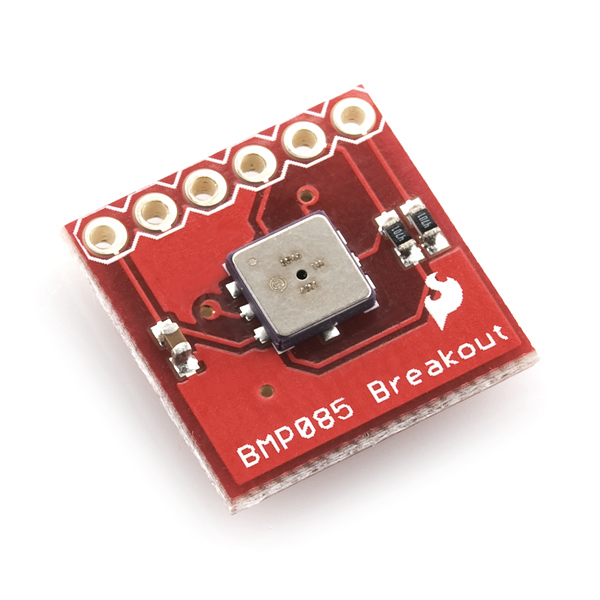
\includegraphics[width=0.3\textwidth]{BMP085}
\caption{The BMP085 barometer.}
\label{fig:BMP085}
\end{figure}

\subsubsection{Cameras}
\label{sec:arch:sensors:cameras}
We have chosen for the Raspberry PI cameras, because they are affordable, of relative good quality, small and light, and they uses few system resources on the Raspberry PI. Because each Raspberry PI can only interface with one camera, we have placed two Raspberry PIs and cameras on the quadcopter.

These cameras are able to film in 1080p resolution with 30 fps, and take still images with 2592 x 1944 resolution.


\begin{figure}[ht]
\centering
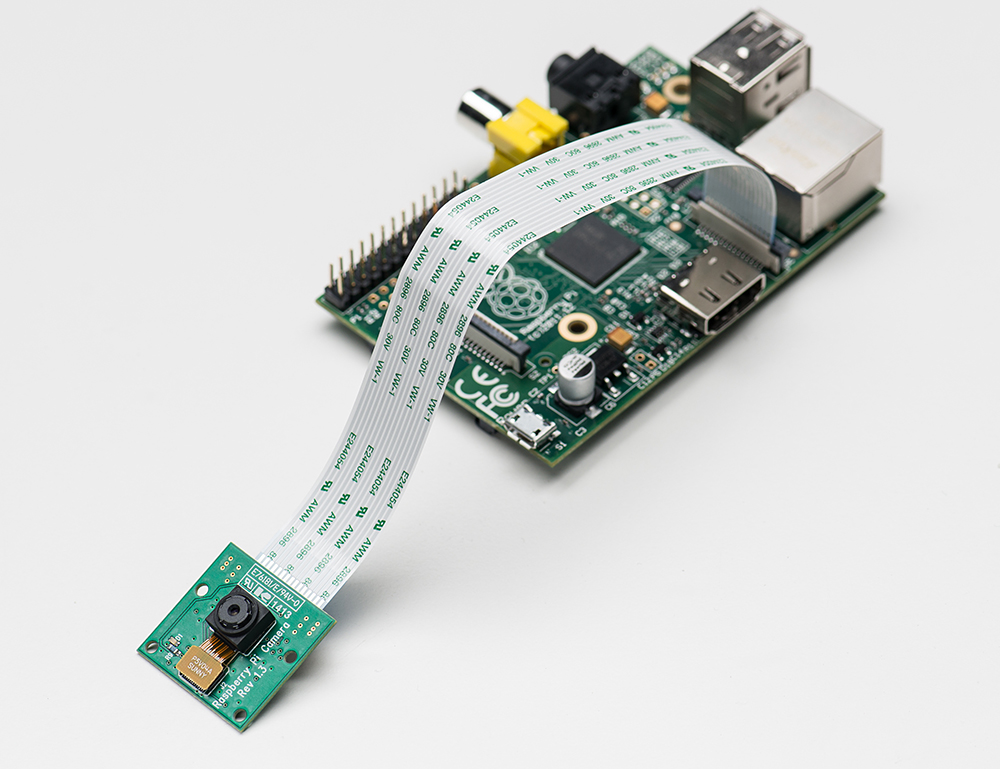
\includegraphics[width=0.6\textwidth]{image03}
\caption{Raspberry PI with camera module.}
\label{fig:raspicamera}
\end{figure}

\subsection{Communication}
\label{sec:arch:comm}
There are many communication-paths, as can be seen in figure \ref{fig:communication}. In this section, these will all be discussed.

\begin{figure}[ht]
\centering
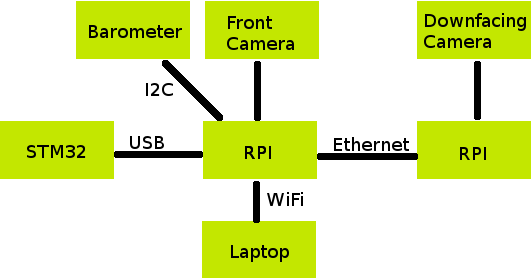
\includegraphics[width=0.6\textwidth]{hwdesign2}
\caption{Overview of different communication protocols.}
\label{fig:communication}
\end{figure}

\subsubsection{Local control and global control}
\label{sec:arch:comm:localglobal}
The local control on the STM32F3Discovery communicates with the first Raspberry PI using an USB-cable. They use the UAVTalk\footnote{\url{http://wiki.openpilot.org/display/Doc/UAVTalk}} protocol, and thus communicate high level objects. Because the UAVTalk protocol is already seamless integrated in the local control (it is also used for communication with the Ground Control Station), all useful pieces of data are available as a UAVObject.

This makes it an extremely powerful interface. Global control algorithms have access to all the information that it available to the local control, and it can influence and override all aspects of the local control by writing new values to these objects.

The interface is also flexible. Currently it uses USB, but UART or other protocols are also possible. The UAVObjects on the local control are also accessible on a laptop and on the other Raspberry PI, using a WiFi or an ethernet connection, thus eliminating the need for a separated (bluetooth) telemetry module.

A presentation on this topic is also available online on \url{http://youtu.be/uEVFPBQtt0U}.

\subsubsection{Raspberry PIs}
\label{sec:arch:comm:raspi}
The two Raspberry PIs on the quadcopter need to be able to communicate, and they do this by a standard ethernet (network) cable. We chose for this option because it is supported out of the box and widely supported, and it is fast. Secondly, it allows the first Raspberry PI to share its WiFi connection easily with the second Raspberry PI, allowing easier remote management.

\subsubsection{Laptop}
\label{sec:arch:comm:laptop}
On the Raspberry PI runs a normal Linux installation, and that gives the option to add a WiFi adaptor so that it can communicate with the outside world using WiFi. We did this, and even shared the internet connection to the second Raspberry PI, so both could easily download and install new software.

\subsubsection{Barometer}
\label{sec:arch:comm:barometer}
The barometer is connected to the first Raspberry PI using I\texttwosuperior C. It is not connected to the STM32F3Discovery, because there where some problems with the I\texttwosuperior C driver in the TauLabs system, that we where unable to properly debug. The Raspberry PI sends the altitude information from the barometer to the STM32F3Discovery using the UAVObjects and the UAVTalk protocol, as discussed in section \ref{sec:arch:comm:localglobal}.

\subsubsection{Camera}
\label{sec:arch:comm:camera}
The cameras are attached to the Raspberry PIs, and use a flatcable for the connection to a CSI\footnote{Camera Serial Interface}-interface.

\section{Software}
\label{sec:software}
To get all this hardware flying, we need some software to control everything. We have software for local and global control, and both will be discussed in this section.

\subsection{Local control}
\label{sec:software:local}
For the local control, we chose for the open source project TauLabs\footnote{\url{https://github.com/TauLabs/TauLabs}}. This project is a fork from the OpenPilot project. We choose for this project, because is was already ported to the hardware we where using (the STM32F3Discovery).

This project provided not only software for the local control, there was also a ``Ground Control Station'' (GCS). This program runs on your computer and communicated with the local control to provide configuration options and means of debugging and monitoring.

\subsection{Global control}
\label{sec:software:global}
We have written our own global control program. This program runs on a Raspberry PI, and is a stripped down version of the GCS provided by TauLabs. This allows it to communicate with the local control using UAVObjects, as is discussed in section \ref{sec:arch:comm:localglobal}. Our global control code is also available on GitHub\footnote{\url{https://github.com/fhp/TauLabs}}.

The global control has a fixed core, and allows functionality to be added by modules. We did not have enough time to write really interesting modules, but we do have some ``proof-of-concept'' modules, which will be discussed next. These plugins show that it is possible to read and write data from/to the local control.

\subsubsection{Recorder plugin}
\label{sec:software:global:recorder}
This plugin monitors the ``Armed'' flag in the ``FlightStatus'' UAVObject, and as soon as the quadcopter gets armed, it starts recording video on both Raspberry PIs. On disarming, the recording stops. This allows us to easily create in-flight footage with the cameras.

\subsubsection{Barometer plugin}
\label{sec:software:global:barometer}
The barometer plugin reads the barometer that is connected to the Raspberry PI using I\texttwosuperior C. It parses the results and writes the resulting altitude information to the ``BaroAltitude'' UAVObject that will then be send to the local control.

\section{Objectives}
\label{sec:objectives}
Here we will discuss the objectives given in the course, and how we handled them.

\subsection{Building Quadcopter and flying}
\label{sec:objectives:building}
We have build our quadcopter, and made fly. See figure \ref{fig:quad} for a photo.

\begin{figure}[ht]
\centering
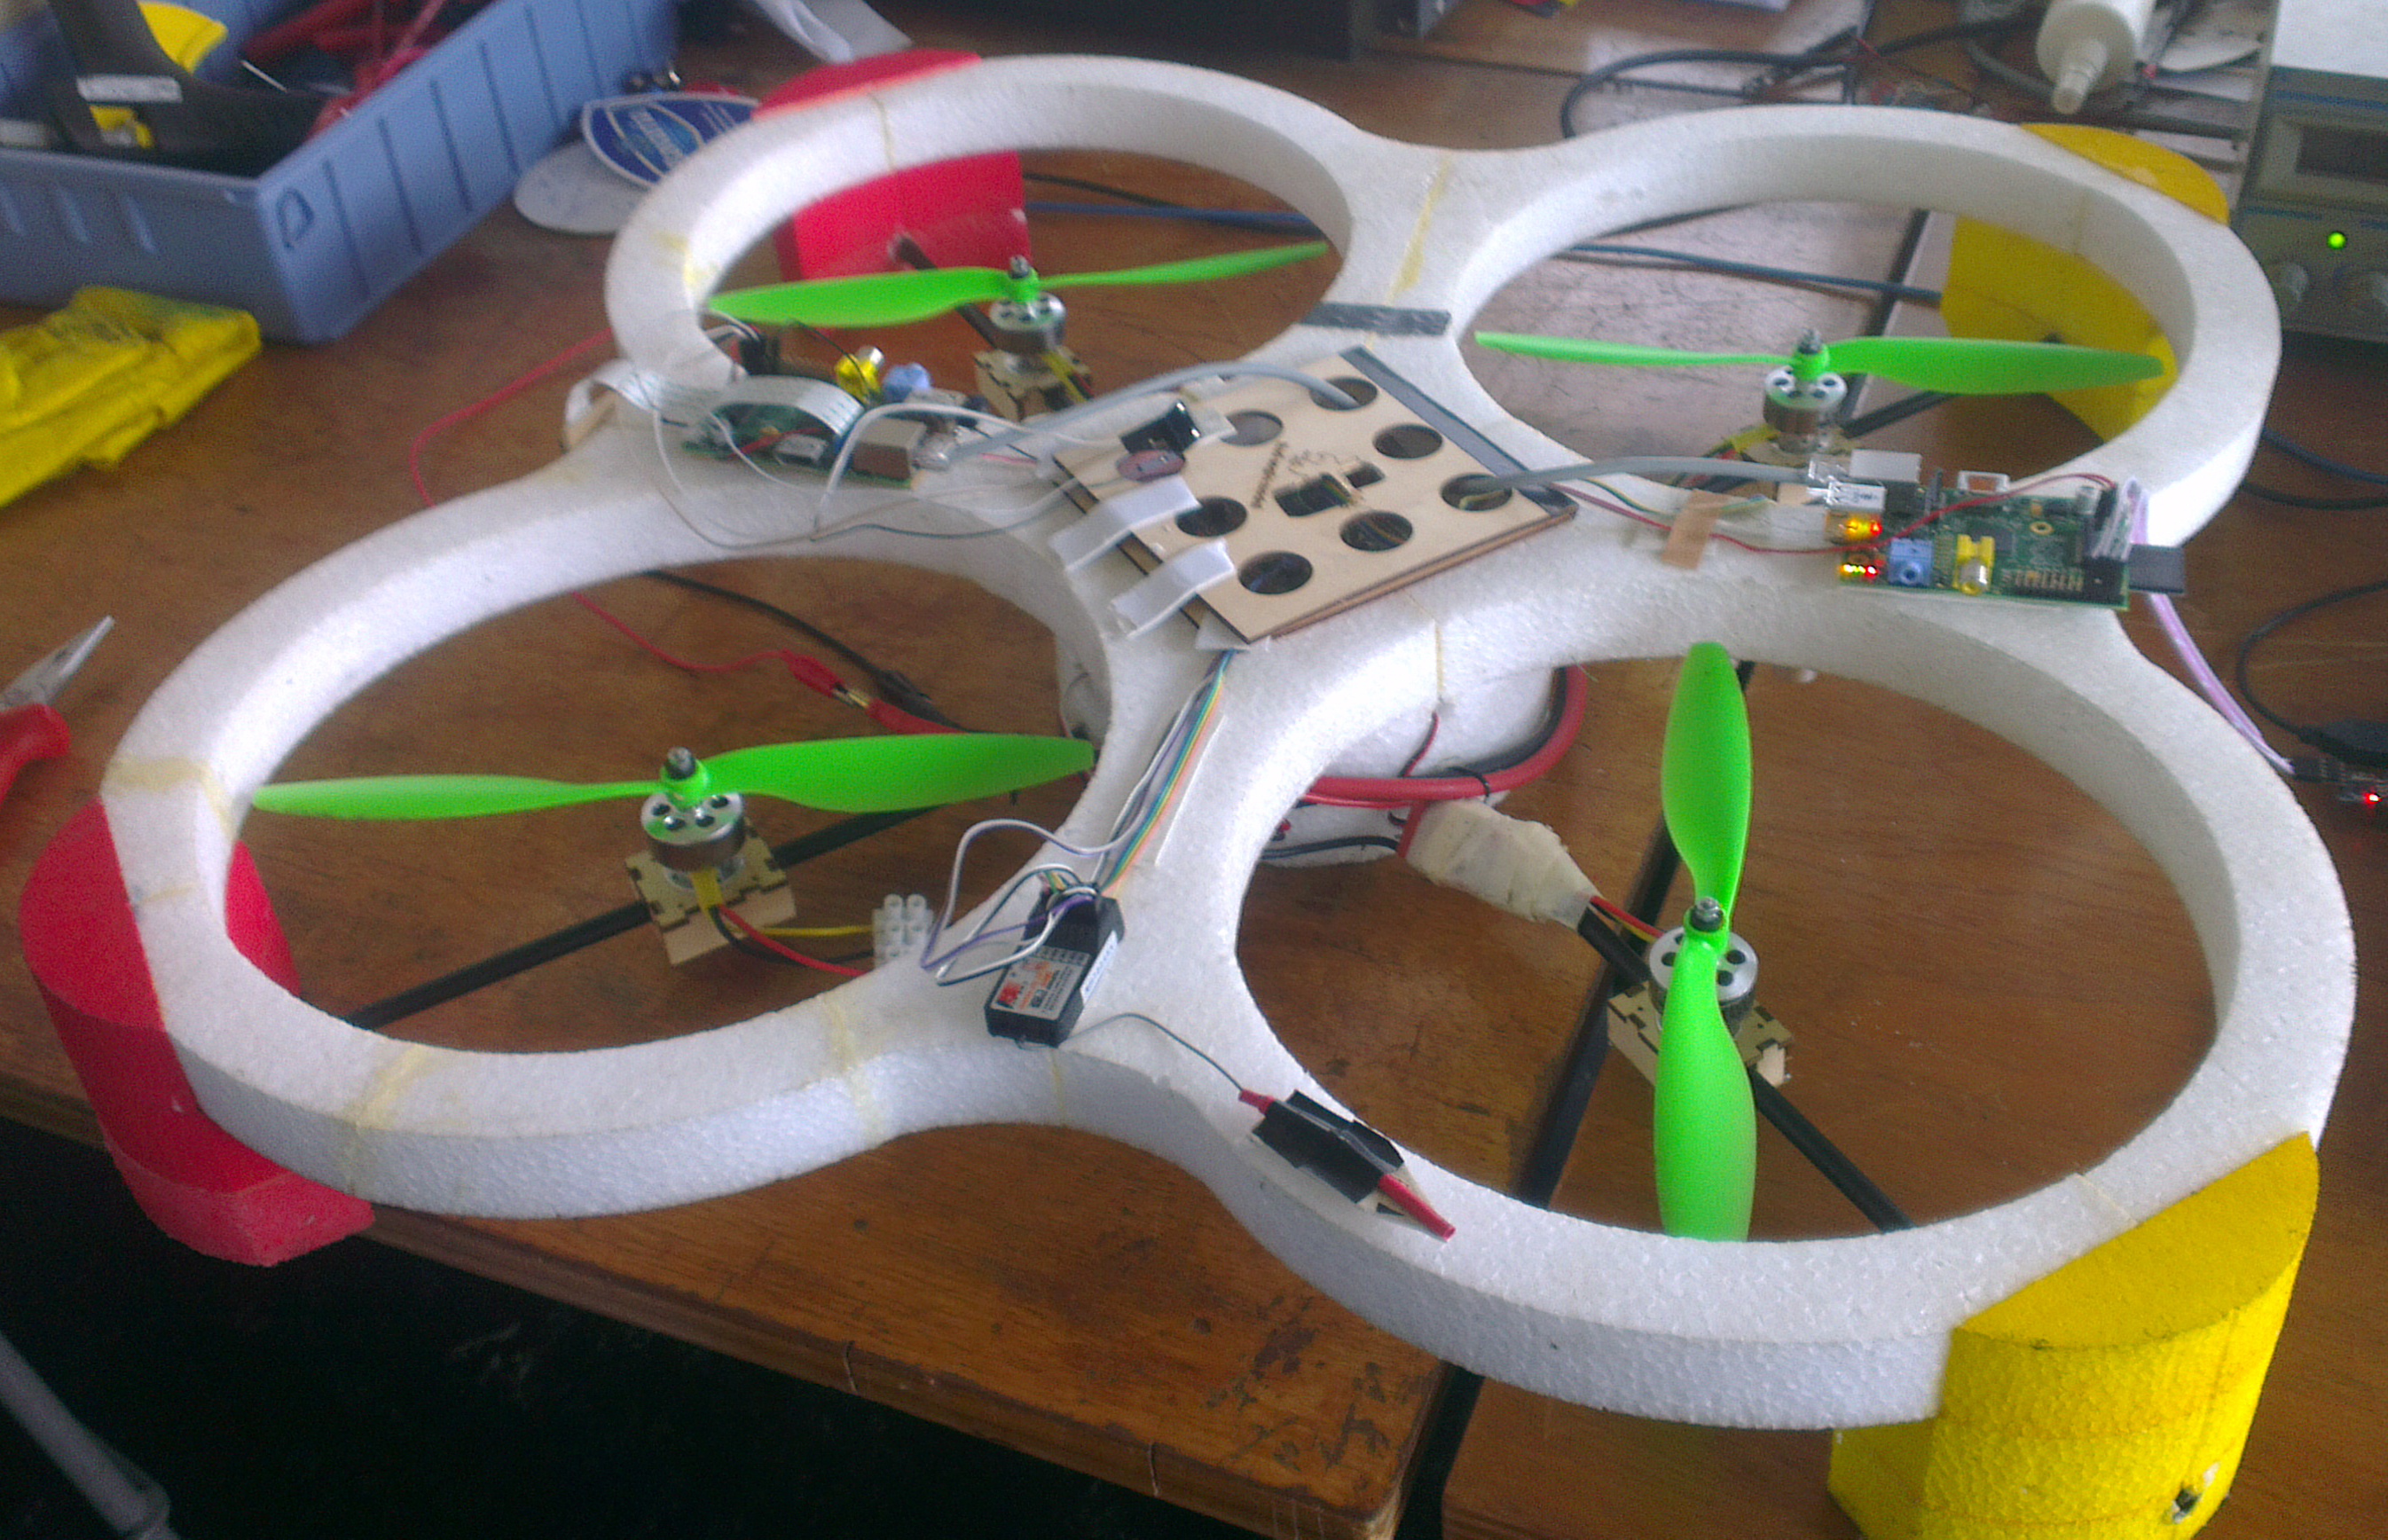
\includegraphics[width=0.6\textwidth]{quad}
\caption{Our quadcopter.}
\label{fig:quad}
\end{figure}

\subsection{Tuning Local control}
\label{sec:objectives:tuning}
We spend a lot of time on PID tuning, but only in the end we found that some of the settings where completely wrong; the direction that the motors where spinning was configured wrong, so yaw corrections resulted in more yaw, crashing the quadcopter. Also one of our speed controllers was not functioning correctly, which led to an unstable quadcopter.

\subsection{Altitude hold}
\label{sec:objectives:altitude}
Altitude hold should have been possible with the barometer installed, but there was no time to actually test this.

\subsection{Autonomous flight}
\label{sec:objectives:autonomous}
We did not manage to get the quadcopter fly autonomously, because it was not stable enough and still needed some manual corrections, and we didn't have altitude hold working.

\subsection{360 degrees panorama}
\label{sec:objectives:panorama}
We where unable to implement this, because we didn't have altitude hold and autonomous flight.

\subsection{Drift correction in horizontal axis}
\label{sec:objectives:drift}
We where unable to implement this, because we didn't have altitude hold and autonomous flight.

\subsection{Face detection}
\label{sec:objectives:face}
% merge with \ref{sec:arch:sensors:cameras}.
During our development period of the quadcopter, the Raspberry PI Foundation has released a camera module (figure \ref{fig:raspicamera}) which fits specifically into Raspberry PI's CSI interface. The camera has a 5 megapixel sensor and supports 1080p, 720p, and 640x480p video. The footprint dimensions are 25 x 20 x 9 mm. Compared to a usb webcam which is widely used for personal computers, the Raspberry PI camera has a relatively smaller size and Raspberry PI has opensource driver for the camera which gives larger throughput in terms of image processing. So we decided to use the Raspberry PI camera as the front facing camera.

The goal of this face detection task is to make the quadcopter follow and track the movement of a human face while flying. We intended to use OpenCV\footnote{\url{http://opencv.org/}} library as a tool to implement the face detection program on Raspberry PI, and after processing the image, we will find the position of the human face relative to the boundary of the image. Based on that position we can decide whether the quadcopter should fly higher or lower, go to the left or to the right. Moreover, and estimated distance of the face from the camera can be calculated by measuring the area of the face within the image taken by the camera. So the quadcopter can track the face when the face is moving away or towards the quadcopter.

However, when we implement the face detection program, we found out that the API from OpenCV library which will invoke the camera to take video is working. Because the Raspberry PI camera uses a different driver model as the conventional usb webcams, the API which is responsible for invoking the camera was not able to locate the camera.

In the Raspbian system, we where provided with two commands to operate the camera; raspivid and raspistill. raspivid is a command line application that allows you to capture video with the camera module, while the application raspistill allows you to capture images.

In order to extract the driver, we looked at the source code of the two applications in the Raspberry PI github repository\footnote{\url{https://github.com/raspberrypi/userland/tree/master/host_applications/linux/apps/raspicam}}. We figured out that the Raspberry PI system uses MMAL functions to communicate with the camera. And we managed to trim down the the camera driver and integrated it into the face detection code. By feeding the haar cascade filter with the image get from the camera, the program is able to detect faces in the image. The output of the program is the coordinate of the face within the image. Figure \ref{fig:raspifaces} shows that the Raspberry PI can successfully detect faces.

\begin{figure}[ht]
\centering
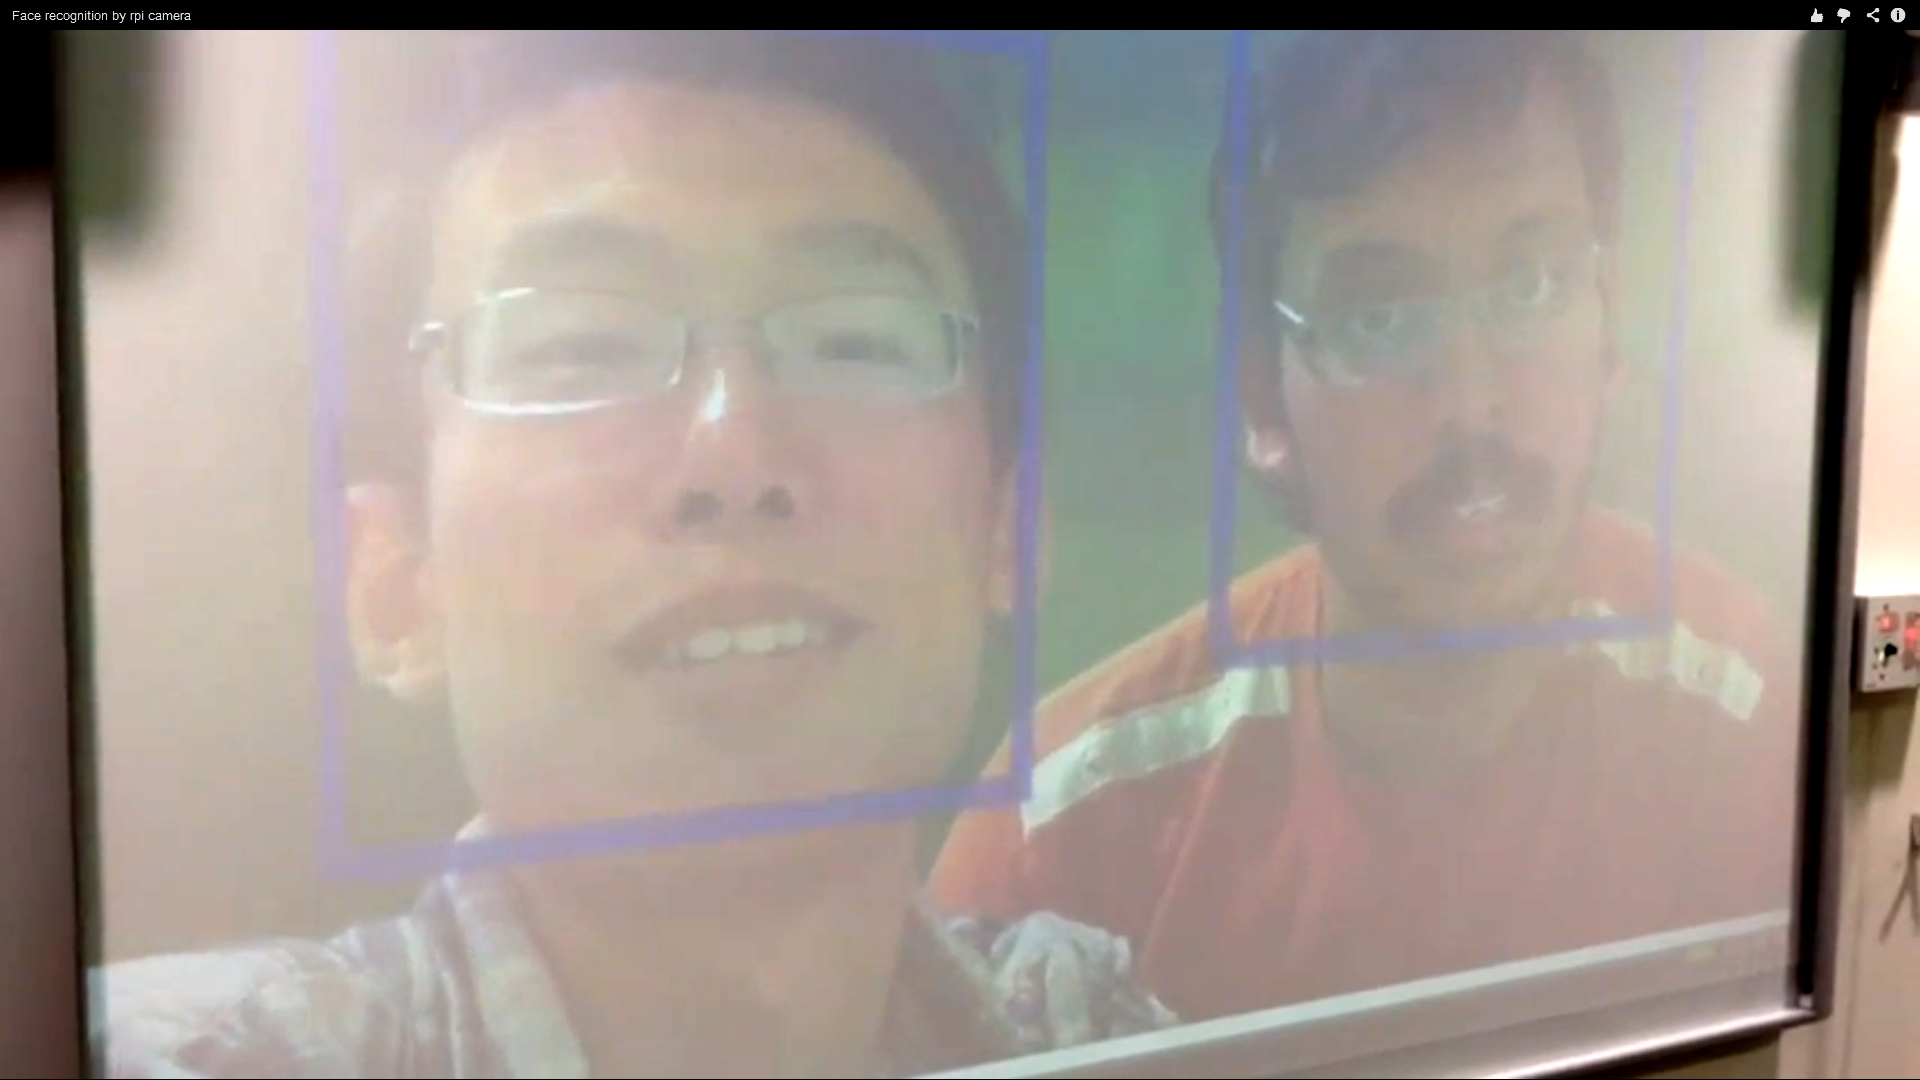
\includegraphics[width=0.6\textwidth]{image02}
\caption{The Raspberry PI has detected faces.}
\label{fig:raspifaces}
\end{figure}

Since the face detection program is based on the haar cascade filter, it will have some drawbacks. First, it will be able to find multiple faces in the camera scene. This may seem to be an advantage, but if two faces appear on the scene, then the quadcopter may not know which one to track, so it may lead to unexpected results. Furthermore, according to the way that haar filter works, it will only detect a face that is placed vertically straight in the image, other orientations will not be detected.

\subsection{Marker identification}
\label{sec:objectives:marker}
The expected output of our marker detection is that the quadcopter can use the front facing camera to detect and recognise some specific markers on the wall, so that it can do some pre-programmed action, that depends on the detected marker. 

As an aerial vehicle, a quadcopter is very susceptible to disturbances from the surrounding. So a quadcopter has to be constantly tuning its position according to the data from the sensors in order to get its stable position. This has disadvantages for the cameras, because for the cameras, a constantly moving quadcopter make the image blurred and therefore make the detection harder. In order to confront this problem, we need to make the markers robust, so that even for a moving quadcopter, the camera can still recognise the markers with high detection rate.

What we use is called ArUco\footnote{\url{http://www.uco.es/investiga/grupos/ava/node/26}}: a minimal library for Augmented Reality applications based on OpenCV. It is a open-source marker detection library developed by University of Cordoba. The library uses markers as shown in figure \ref{fig:markers}.

\begin{figure}[ht]
\centering
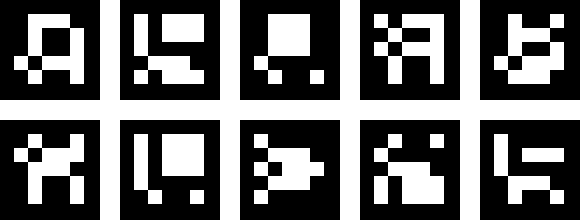
\includegraphics[width=0.8\textwidth]{image00}
\caption{ArUco markers}
\label{fig:markers}
\end{figure}

Each marker has an internal code given by 5 words of 5 bits each (as shown in figure \ref{fig:markerstructure}). The codification employed is a slight modification of the Hamming Code. In total, each word has only 2 bits of information out of the 5 bits employed. The other 3 are employed for error detection. As a consequence, we can have up to 1024 different ids. With the help of Hamming coding, the marker is able to tolerate more errors, and the robustness of the detection is increased.

\begin{figure}[ht]
\centering
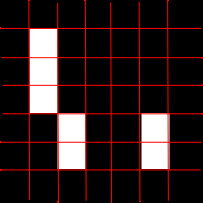
\includegraphics[width=0.25\textwidth]{image04}
\caption{Marker structure}
\label{fig:markerstructure}
\end{figure}

The main difference with the Hamming Code is that the first bit (parity of bits 3 and 5) is inverted. So, the id 0 (which in hamming code is 00000) becomes 10000 in our codification. The idea is to prevent a completely black rectangle from being a valid marker id with the goal of reducing the likelihood of false positives with objects of the environment.

Since we already have the experience of face detection program, we successfully integrated the marker detection code with raspberry pi camera driver as well. As a result of the program it can detect the marker printed on a paper as well as knowing the corresponding id of this marker (figure \ref{fig:markerdetected}). Based on the id, the quadcopter can be assigned to do some pre-defined actions like turn around or go forward, etc.

\begin{figure}[ht]
\centering
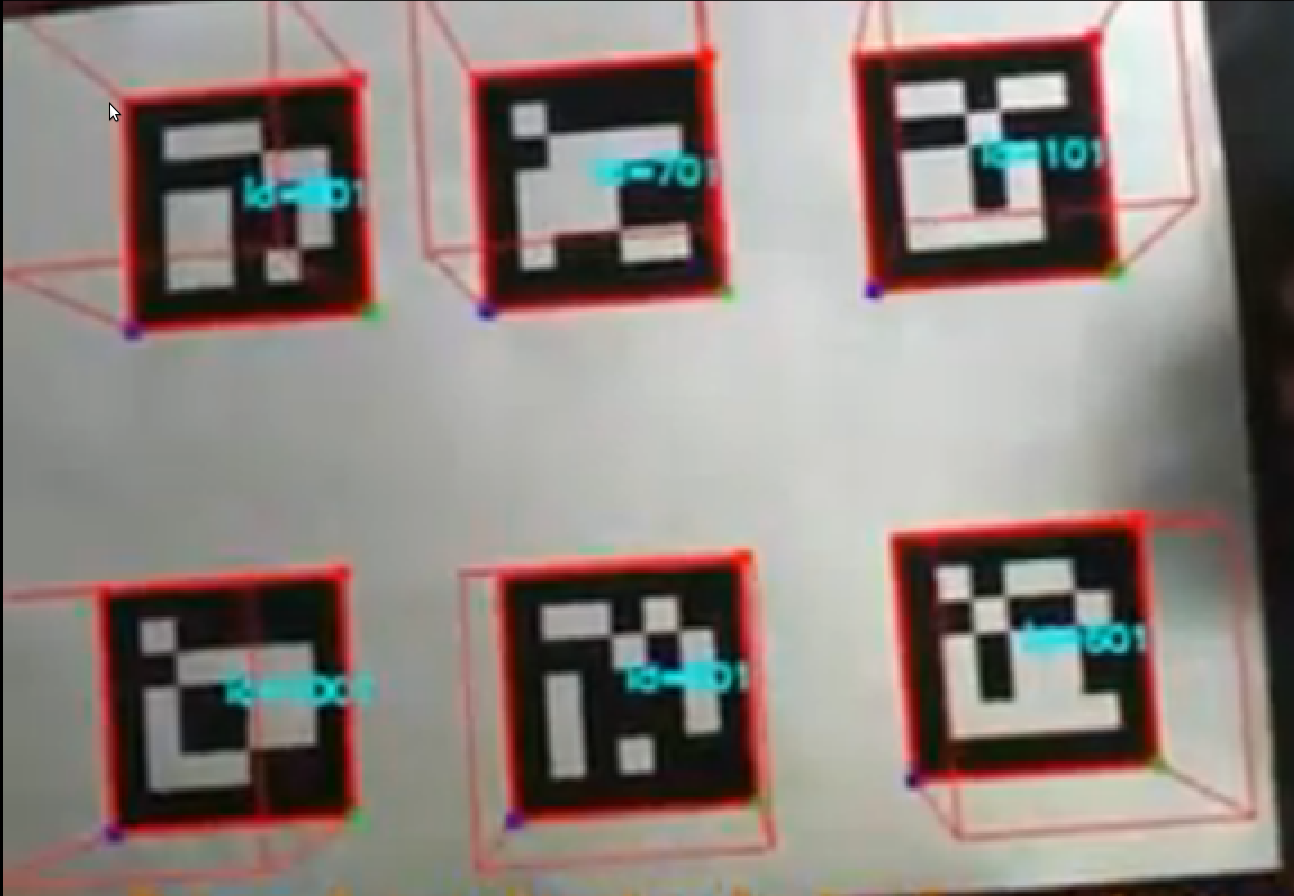
\includegraphics[width=0.6\textwidth]{image05}
\caption{Detected markers}
\label{fig:markerdetected}
\end{figure}

\FloatBarrier
\hbox{}
\newpage
\appendix

\section{Who did what?}
\subsection{Hardware}
\begin{tabular}{ll}
Building the basic quadcopter & Stef, Sunil, Qian \\
Basic PID tuning & Stef, Sunil, Qian \\
More PID tuning & Stef \\
Installing the cameras & Stef, Sunil \\
Installing the ultrasound sensor & Stef, Sunil \\
Installing the battery monitor & Stef \\
Installing the barometer & Stef \\
\end{tabular}

\subsection{Software}
\begin{tabular}{ll}
UAVTalk on Raspberry PI & Stef \\
Global control & Stef \\
Face recognition & Qian \\
Marker recognition & Qian \\
Sonar integration on local control & Sunil \\
\end{tabular}

\subsection{Report}
\begin{tabular}{ll}
Ultrasound (section \ref{sec:arch:sensors:ultrasound}) & Sunil \\
Face detection (section \ref{sec:objectives:face}) & Qian \\
Marker detection (section \ref{sec:objectives:marker}) & Qian \\
The other sections & Stef \\
\end{tabular}

\newpage
\section{Partlist}
Here follows a list of all the parts and components that we have used while building this quadcopter.

In the total, all currencies have been converted to euro's.

\begin{tabular}{llr@{.}lr@{.}l}
  & \multicolumn{3}{l}{HobbyKing \#2006549947} \\ % Stef
1 & Extra Large EPP Quadcopter Frame 450mm & \$27&81 & \$27&81 \\
1 & Turnigy 5000mAh 3S 30C Lipo Pack & \$40&87 & \$40&87 \\
2 & Slow Fly Electric Prop 1045 SF & \$3&57 &  \$7&14 \\
  & Shipping & \multicolumn{2}{c}{--} & \$7&93 \\
\hline % euro: 67.32

  & \multicolumn{3}{l}{HobbyKing \#2006549967} \\ % Stef
1 & Polymax 5.5mm Gold Connectors 10 pairs & \$5&39 & \$5&39 \\
2 & Slow Fly Electric Prop 1045R SF & \$3&53 & \$7&06 \\
4 & Turnigy DST-1200 Brushless Bell Motor 1200kv & \$7&16 & \$28&64 \\
4 & HobbyKing Red Brick 20A ESC & \$7&18 & \$28&72 \\
  & Shipping & \multicolumn{2}{c}{--} & \$6&01 \\
\hline % euro: 60.47

  & \multicolumn{3}{l}{Deal eXtreme \#130402001086499449} \\ % Stef
2 & HC-SR04 Ultrasonic Sensor & \$3&20 & \$6&40 \\
1 & JY-MCU Bluetooth Serial Port Module & \$8&20 & \$8&20 \\
\hline % euro: 11.74

  & \multicolumn{3}{l}{Deal eXtreme \#130402001088428719} \\ % Stef
1 & Super Mini Bluetooth 2.0 Adapter Dongle & \$1&80 & \$1&80 \\
\hline % euro: 1.45

  & \multicolumn{3}{l}{Dick Best \#130506-231645-1685} \\ % Stef
2 & Header 2x28 polig Female Recht Verguld & \texteuro2&00 & \texteuro4&00 \\
2 & Header 2x11 polig Female & \texteuro1&20 & \texteuro2&40 \\
1 & Header  15 polig Female & \texteuro0&90 & \texteuro0&90 \\
  & Shipping & \multicolumn{2}{c}{--} & \texteuro2&25 \\
\hline % euro: 9.55

  & \multicolumn{3}{l}{Farnell \#ORP116530} \\ % Stef
2 & Raspberry PI, Model B, 512MB & \pounds28&31 & \pounds56&62 \\
2 & Raspberry PI Camera Board & \pounds20&04 & \pounds40&08 \\
\hline % euro: 114.37

  & \multicolumn{3}{l}{HobbyKing \#2007104426} \\ % Stef
1 & ZIPPY Flightmax 4200mAh 3S1P 30C & \$32&96 & \$32&96 \\
  & Shipping & \multicolumn{2}{c}{--} & \$6&01 \\
\hline % euro: 30.00

  & \multicolumn{3}{l}{Ebay \#434632019023} \\ % Stef
1 & BMP085 Barometric Digital Pressure Sensor & \$4&09 & \$4&09 \\
\hline % euro 3.01

  & \multicolumn{3}{l}{Ebay \#874439470014} \\ % Stef
1 & Low Voltage Buzzer For 2s 3s Lipo Battery & \$1&96 & \$1&96 \\
% euro 1.53

\hline
\hline
  & \textbf{Subtotal} & \multicolumn{2}{c}{} & \texteuro 299&44 \\
\end{tabular}
% Total Stef: euro 299.44

\begin{tabular}{llr@{.}lr@{.}l}
  & Previous page & \multicolumn{2}{c}{} & \texteuro 299&44 \\
\hline

  & \multicolumn{3}{l}{Ebay \#160991485511} \\ % Sunil
1 & STM32F3 Discovery & \texteuro13&05 & \texteuro13&05 \\
  & Shipping & \multicolumn{2}{c}{--} & \texteuro5&00 \\
\hline % euro 18.05

  & \multicolumn{3}{l}{HobbyKing \#2006549967} \\ % Sunil
4 & Turnigy DST-1200 Brushless Bell Motor 1200kv & \$6&37 & \$25&48 \\
1 & Nylon XT60 Connectors & \$3&29 & \$3&29 \\
1 & HXT 4mm Gold Connector & \$4&12 & \$4&12 \\
  & Customs & \multicolumn{2}{c}{--} & \texteuro18&20 \\
  & Shipping & \multicolumn{2}{c}{--} & \$9&99 \\
\hline % euro: 50.00

  & \multicolumn{3}{l}{Amazon \#304-1140681-4631520} \\ % Sunil
1 & TP-Link TL-WN725N Wireless N USB-Adapter & \texteuro9&72  & \texteuro9&72 \\
  & Shipping & \multicolumn{2}{c}{--} & \texteuro4&69 \\
\hline % euro 14.41

% Total Sunil: 82.46

  & \multicolumn{3}{l}{Ebay \#160991485511} \\ % Qian
1 & STM32F3 Discovery & \pounds20&98  & \pounds20&98 \\
  & Shipping & \multicolumn{2}{c}{--} & \pounds10&99 \\
% euro 37.84

% Total Qian 37.84

\hline
\hline
  & \textbf{Total} & \multicolumn{2}{c}{} & \texteuro 419&74 \\

\end{tabular}
\end{document}
